\documentclass[a4paper,11pt]{exam}
%\printanswers % pour imprimer les réponses (corrigé)
\noprintanswers % Pour ne pas imprimer les réponses (énoncé)
\addpoints % Pour compter les points
% \noaddpoints % pour ne pas compter les points
%\qformat{\textbf{\thequestion ) } }
%\qformat{\textbf{\thequestion )}} % Pour définir le style des questions (facultatif)
\usepackage{color} % définit une nouvelle couleur
\shadedsolutions % définit le style des réponses
% \framedsolutions % définit le style des réponses
\definecolor{SolutionColor}{rgb}{0.8,0.9,1} % bleu ciel
\renewcommand{\solutiontitle}{\noindent\textbf{Solution:}\par\noindent} % Définit le titre des solutions
\usepackage{gensymb}



\makeatletter

\def\maketitle{{\centering%
	\par{\huge\textbf{\@title}}%
	\par{\@date}%
	\par}}


\renewcommand{\thesubsection}{\Alph{subsection}.}   

\makeatother

\lhead{NOM Pr\'enom :}
\rhead{\textbf{Les r\'eponses doivent \^etre justifi\'ees et r\'edig\'ees}}
\cfoot{\thepage / \pageref{LastPage}}


%\usepackage{../../pas-math}
%\usepackage{../../moncours}


%\usepackage{pas-cours}
%-------------------------------------------------------------------------------
%          -Packages nécessaires pour écrire en Français et en UTF8-
%-------------------------------------------------------------------------------
\usepackage[utf8]{inputenc}
\usepackage[frenchb]{babel}
%\usepackage{numprint}
\usepackage[T1]{fontenc}
%\usepackage{lmodern}
\usepackage{textcomp}
\usepackage[french, boxed]{algorithm2e}
\usepackage{hyperref}


%-------------------------------------------------------------------------------

%-------------------------------------------------------------------------------
%                          -Outils de mise en forme-
%-------------------------------------------------------------------------------
\usepackage{hyperref}
\hypersetup{pdfstartview=XYZ}
%\usepackage{enumerate}
\usepackage{graphicx}
\usepackage{multicol}
\usepackage{tabularx}
\usepackage{multirow}
\usepackage{color}
\usepackage{eurosym}


\usepackage{anysize} %%pour pouvoir mettre les marges qu'on veut
%\marginsize{2.5cm}{2.5cm}{2.5cm}{2.5cm}

\usepackage{indentfirst} %%pour que les premier paragraphes soient aussi indentés
\usepackage{verbatim}
\usepackage{enumitem}
\usepackage{booktabs}
\usepackage[usenames,dvipsnames,svgnames,table]{xcolor}

\usepackage{variations}

%-------------------------------------------------------------------------------


%-------------------------------------------------------------------------------
%                  -Nécessaires pour écrire des mathématiques-
%-------------------------------------------------------------------------------
\usepackage{amsfonts}
\usepackage{amssymb}
\usepackage{amsmath}
\usepackage{amsthm}
\usepackage{tikz}
\usepackage{xlop}
\usepackage[output-decimal-marker={,}]{siunitx}
%-------------------------------------------------------------------------------

%-------------------------------------------------------------------------------
%                  -Nécessaires pour écrire des formules chimiquess-
%-------------------------------------------------------------------------------

\usepackage[version=4]{mhchem}

%-------------------------------------------------------------------------------
% Pour pouvoir exploiter les fichiers directement dans beamer
\newcommand{\pause}{\ }
%-------------------------------------------------------------------------------
%                    - Mise en forme avancée
%-------------------------------------------------------------------------------

\usepackage{ifthen}
\usepackage{ifmtarg}


\newcommand{\ifTrue}[2]{\ifthenelse{\equal{#1}{true}}{#2}{$\qquad \qquad$}}

%\newcommand{\kword}[1]{\textcolor{red}{\underline{#1}}}
%-------------------------------------------------------------------------------

%-------------------------------------------------------------------------------
%                     -Mise en forme d'exercices-
%-------------------------------------------------------------------------------
%\newtheoremstyle{exostyle}
%{\topsep}% espace avant
%{\topsep}% espace apres
%{}% Police utilisee par le style de thm
%{}% Indentation (vide = aucune, \parindent = indentation paragraphe)
%{\bfseries}% Police du titre de thm
%{.}% Signe de ponctuation apres le titre du thm
%{ }% Espace apres le titre du thm (\newline = linebreak)
%{\thmname{#1}\thmnumber{ #2}\thmnote{. \normalfont{\textit{#3}}}}% composants du titre du thm : \thmname = nom du thm, \thmnumber = numéro du thm, \thmnote = sous-titre du thm

%\theoremstyle{exostyle}
%\newtheorem{exercice}{Exercice}
%
%\newenvironment{questions}{
%\begin{enumerate}[\hspace{12pt}\bfseries\itshape a.]}{\end{enumerate}
%} %mettre un 1 à la place du a si on veut des numéros au lieu de lettres pour les questions 
%-------------------------------------------------------------------------------

%-------------------------------------------------------------------------------
%                    - Mise en forme de tableaux -
%-------------------------------------------------------------------------------

\renewcommand{\arraystretch}{1.7}

\setlength{\tabcolsep}{1.2cm}

%-------------------------------------------------------------------------------



%-------------------------------------------------------------------------------
%                    - Racourcis d'écriture -
%-------------------------------------------------------------------------------
%Droites
\newcommand{\dte}[1]{$(#1)$}
\newcommand{\fig}[1]{figure $#1$}
\newcommand{\sym}{symétrique}
\newcommand{\syms}{symétriques}
\newcommand{\asym}{axe de symétrie}
\newcommand{\asyms}{axes de symétrie}
\newcommand{\seg}[1]{$[#1]$}
\newcommand{\monAngle}[1]{$\widehat{#1}$}
\newcommand{\bissec}{bissectrice}
\newcommand{\mediat}{médiatrice}
\newcommand{\ddte}[1]{$[#1)$}


% Angles orientés (couples de vecteurs)
\newcommand{\aopp}[2]{(\vec{#1}, \vec{#2})} %Les deuc vecteurs sont positifs
\newcommand{\aopn}[2]{(\vec{#1}, -\vec{#2})} %Le second vecteur est négatif
\newcommand{\aonp}[2]{(-\vec{#1}, \vec{#2})} %Le premier vecteur est négatif
\newcommand{\aonn}[2]{(-\vec{#1}, -\vec{#2})} %Les deux vecteurs sont négatifs

%Ensembles mathématiques
\newcommand{\naturels}{\mathbb{N}} %Nombres naturels
\newcommand{\relatifs}{\mathbb{Z}} %Nombres relatifs
\newcommand{\rationnels}{\mathbb{Q}} %Nombres rationnels
\newcommand{\reels}{\mathbb{R}} %Nombres réels
\newcommand{\complexes}{\mathbb{C}} %Nombres complexes


%Intégration des parenthèses aux cosinus
\newcommand{\cosP}[1]{\cos\left(#1\right)}
\newcommand{\sinP}[1]{\sin\left(#1\right)}


%Probas stats
\newcommand{\stat}{statistique}
\newcommand{\stats}{statistiques}


\newcommand{\homo}{homothétie}
\newcommand{\homos}{homothéties}


\newcommand{\mycoord}[3]{(\textcolor{red}{\num{#1}} ; \textcolor{Green}{\num{#2}} ; \textcolor{blue}{\num{#3}})}
%-------------------------------------------------------------------------------

%-------------------------------------------------------------------------------
%                    - Mise en page -
%-------------------------------------------------------------------------------

\newcommand{\twoCol}[1]{\begin{multicols}{2}#1\end{multicols}}


\setenumerate[1]{font=\bfseries,label=\textit{\alph*})}
\setenumerate[2]{font=\bfseries,label=\arabic*)}


%-------------------------------------------------------------------------------
%                    - Elements cours -
%-------------------------------------------------------------------------------

%Correction d'exercice
\newcommand{\exoSec}[2]{\subsection*{Exercice #1 page #2}}
%-------------------------------------------------------------------------------
%                    - raccourcis d'écriture -
%-------------------------------------------------------------------------------

%Mise en évidence de termes clés
\newcommand{\mykw}[1]{\textcolor{red}{\underline{\textbf{#1}}}}

%Exercices
\newcommand{\exo}[2]{exercice #1 page #2}
\newcommand{\Exo}[2]{Exercice #1 page #2}

\renewcommand{\pause}{\ }

%Intervalles
\newcommand{\interOO}[2]{$]$#1 , #2$[$}
\newcommand{\interOF}[2]{$]$#1 , #2$]$}
\newcommand{\interFO}[2]{$[$#1 , #2$[$}
\newcommand{\interFF}[2]{$[$#1 , #2$]$}



%\usepackage{fullpage}
\author{\ }
\date{24 Septembre 2018}
\title{Sciences Physiques : DS n° 1}


\begin{document}
%	\usepackage{fancyhdr}
%	
%	\pagestyle{fancy}
%	\fancyhf{}
	%\rhead{Share\LaTeX}

	\maketitle
	
\begin{small}
	\begin{center}
		\begin{tabular}{|@{\ }l@{}|@{\ }c@{\ }|}
			\hline
			\textbf{Compétence} & \textbf{Maitrise} \\
			\hline
			Exploiter des mesures de masse volumique pour différencier des espèces chimiques.\ &  \ \ \ \\
			\hline	
		\end{tabular}
	\end{center}
\end{small}	
	
	
%\vspace*{-0.5cm}	

%\section{\'Equations de réaction}

Ajuster les équations de réactions suivantes :
\begin{questions}
	\question $CH_4 + ....O_2 \rightarrow ....CO_2 + ....H_2O$
	
	\question $C_7H_{16} + ....O_2 \rightarrow ....CO_2 + ....H_2O$	
	
	\question $C_6H_{2}O + ....O_2 \rightarrow ....CO_2 + ....H_2O$
\end{questions}


%\section{À chaque modèle sa formule}
\begin{questions}
	\question \'A partir de ces dessins de modèles, donner la formule des molécules suivantes.

	\begin{center}
		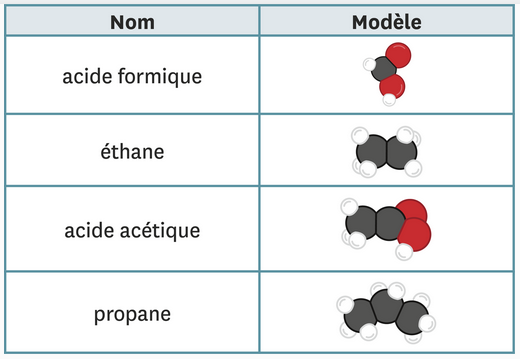
\includegraphics[scale=0.6]{img/exemples}
	\end{center}
	\fillwithdottedlines{2cm}
	
\end{questions}

%Seul l'\ref{ex:qcm} est à faire sur le sujet. Le soin et la qualité de rédaction sont pris en compte dans la notation.


\section{Quels atomes dans cette particule ? (4 points)}\label{ex:particule}



\begin{questions}
	\question[4] Pour chaque espèce chimique, indiquer le type d'atome, le nombre d'atomes de chaque type et le nombre total d'atomes qu'elle contient.
	 
	\begin{multicols}{4}
		\begin{itemize}
			\item $CO_2$
			\item $H_2$
			\item $CH_4$
			\item $O_2$
			\item $C_4H_{10} $
			\item $C_6H_{12} O_6$
			\item $C$
			\item $H_2O$
		\end{itemize}
	\end{multicols}

	\begin{solution}
		\begin{tabular}{|@{\ }c@{\ }|@{\ }c@{\ }|@{\ }c@{\ }|@{\ }c@{\ }|@{\ }c@{\ }|}
			\hline
			Molécule         & Nombre d'atomes & Nombre d'atomes & Nombre d'atomes & Nombre total \\ 
			& de carbone      & d'hydrogène     & d'oxygène       & d'atomes         \\ \hline
			$CO_2$           & 1               & 0               & 2               & 3               \\ \hline
			$H_2$            & 0               & 2               & 0               & 2               \\ \hline
			$CH_4$           & 1               & 4               & 0               & 5               \\ \hline
			$O_2$            & 0               & 0               & 2               & 2               \\ \hline
			$C_4H_{10}$      & 4               & 10              & 0               & 14              \\ \hline
			$C_6H_{12}O_{6}$ & 6               & 12              & 6               & 24              \\ \hline
			$C$              & 1               & 0               & 0               & 1               \\ \hline
			$H_2O$           & 0               & 2               & 1               & 3               \\ \hline
		\end{tabular}
	\end{solution}
	
\end{questions}

%\newpage





\documentclass[12pt,a4paper]{article}

%\usepackage[left=1.5cm,right=1.5cm,top=1cm,bottom=2cm]{geometry}
\usepackage[in, plain]{fullpage}
\usepackage{array}
%\usepackage{../../pas-math}
\usepackage{../../moncours}



%-------------------------------------------------------------------------------
%          -Packages nécessaires pour écrire en Français et en UTF8-
%-------------------------------------------------------------------------------
\usepackage[utf8]{inputenc}
\usepackage[frenchb]{babel}
%\usepackage{numprint}
\usepackage[T1]{fontenc}
%\usepackage{lmodern}
\usepackage{textcomp}
\usepackage[french, boxed]{algorithm2e}
\usepackage{hyperref}


%-------------------------------------------------------------------------------

%-------------------------------------------------------------------------------
%                          -Outils de mise en forme-
%-------------------------------------------------------------------------------
\usepackage{hyperref}
\hypersetup{pdfstartview=XYZ}
%\usepackage{enumerate}
\usepackage{graphicx}
\usepackage{multicol}
\usepackage{tabularx}
\usepackage{multirow}
\usepackage{color}
\usepackage{eurosym}


\usepackage{anysize} %%pour pouvoir mettre les marges qu'on veut
%\marginsize{2.5cm}{2.5cm}{2.5cm}{2.5cm}

\usepackage{indentfirst} %%pour que les premier paragraphes soient aussi indentés
\usepackage{verbatim}
\usepackage{enumitem}
\usepackage{booktabs}
\usepackage[usenames,dvipsnames,svgnames,table]{xcolor}

\usepackage{variations}

%-------------------------------------------------------------------------------


%-------------------------------------------------------------------------------
%                  -Nécessaires pour écrire des mathématiques-
%-------------------------------------------------------------------------------
\usepackage{amsfonts}
\usepackage{amssymb}
\usepackage{amsmath}
\usepackage{amsthm}
\usepackage{tikz}
\usepackage{xlop}
\usepackage[output-decimal-marker={,}]{siunitx}
%-------------------------------------------------------------------------------

%-------------------------------------------------------------------------------
%                  -Nécessaires pour écrire des formules chimiquess-
%-------------------------------------------------------------------------------

\usepackage[version=4]{mhchem}

%-------------------------------------------------------------------------------
% Pour pouvoir exploiter les fichiers directement dans beamer
\newcommand{\pause}{\ }
%-------------------------------------------------------------------------------
%                    - Mise en forme avancée
%-------------------------------------------------------------------------------

\usepackage{ifthen}
\usepackage{ifmtarg}


\newcommand{\ifTrue}[2]{\ifthenelse{\equal{#1}{true}}{#2}{$\qquad \qquad$}}

%\newcommand{\kword}[1]{\textcolor{red}{\underline{#1}}}
%-------------------------------------------------------------------------------

%-------------------------------------------------------------------------------
%                     -Mise en forme d'exercices-
%-------------------------------------------------------------------------------
%\newtheoremstyle{exostyle}
%{\topsep}% espace avant
%{\topsep}% espace apres
%{}% Police utilisee par le style de thm
%{}% Indentation (vide = aucune, \parindent = indentation paragraphe)
%{\bfseries}% Police du titre de thm
%{.}% Signe de ponctuation apres le titre du thm
%{ }% Espace apres le titre du thm (\newline = linebreak)
%{\thmname{#1}\thmnumber{ #2}\thmnote{. \normalfont{\textit{#3}}}}% composants du titre du thm : \thmname = nom du thm, \thmnumber = numéro du thm, \thmnote = sous-titre du thm

%\theoremstyle{exostyle}
%\newtheorem{exercice}{Exercice}
%
%\newenvironment{questions}{
%\begin{enumerate}[\hspace{12pt}\bfseries\itshape a.]}{\end{enumerate}
%} %mettre un 1 à la place du a si on veut des numéros au lieu de lettres pour les questions 
%-------------------------------------------------------------------------------

%-------------------------------------------------------------------------------
%                    - Mise en forme de tableaux -
%-------------------------------------------------------------------------------

\renewcommand{\arraystretch}{1.7}

\setlength{\tabcolsep}{1.2cm}

%-------------------------------------------------------------------------------



%-------------------------------------------------------------------------------
%                    - Racourcis d'écriture -
%-------------------------------------------------------------------------------
%Droites
\newcommand{\dte}[1]{$(#1)$}
\newcommand{\fig}[1]{figure $#1$}
\newcommand{\sym}{symétrique}
\newcommand{\syms}{symétriques}
\newcommand{\asym}{axe de symétrie}
\newcommand{\asyms}{axes de symétrie}
\newcommand{\seg}[1]{$[#1]$}
\newcommand{\monAngle}[1]{$\widehat{#1}$}
\newcommand{\bissec}{bissectrice}
\newcommand{\mediat}{médiatrice}
\newcommand{\ddte}[1]{$[#1)$}


% Angles orientés (couples de vecteurs)
\newcommand{\aopp}[2]{(\vec{#1}, \vec{#2})} %Les deuc vecteurs sont positifs
\newcommand{\aopn}[2]{(\vec{#1}, -\vec{#2})} %Le second vecteur est négatif
\newcommand{\aonp}[2]{(-\vec{#1}, \vec{#2})} %Le premier vecteur est négatif
\newcommand{\aonn}[2]{(-\vec{#1}, -\vec{#2})} %Les deux vecteurs sont négatifs

%Ensembles mathématiques
\newcommand{\naturels}{\mathbb{N}} %Nombres naturels
\newcommand{\relatifs}{\mathbb{Z}} %Nombres relatifs
\newcommand{\rationnels}{\mathbb{Q}} %Nombres rationnels
\newcommand{\reels}{\mathbb{R}} %Nombres réels
\newcommand{\complexes}{\mathbb{C}} %Nombres complexes


%Intégration des parenthèses aux cosinus
\newcommand{\cosP}[1]{\cos\left(#1\right)}
\newcommand{\sinP}[1]{\sin\left(#1\right)}


%Probas stats
\newcommand{\stat}{statistique}
\newcommand{\stats}{statistiques}


\newcommand{\homo}{homothétie}
\newcommand{\homos}{homothéties}


\newcommand{\mycoord}[3]{(\textcolor{red}{\num{#1}} ; \textcolor{Green}{\num{#2}} ; \textcolor{blue}{\num{#3}})}
%-------------------------------------------------------------------------------

%-------------------------------------------------------------------------------
%                    - Mise en page -
%-------------------------------------------------------------------------------

\newcommand{\twoCol}[1]{\begin{multicols}{2}#1\end{multicols}}


\setenumerate[1]{font=\bfseries,label=\textit{\alph*})}
\setenumerate[2]{font=\bfseries,label=\arabic*)}


%-------------------------------------------------------------------------------
%                    - Elements cours -
%-------------------------------------------------------------------------------

%Correction d'exercice
\newcommand{\exoSec}[2]{\subsection*{Exercice #1 page #2}}
%-------------------------------------------------------------------------------
%                    - raccourcis d'écriture -
%-------------------------------------------------------------------------------

%Mise en évidence de termes clés
\newcommand{\mykw}[1]{\textcolor{red}{\underline{\textbf{#1}}}}

%Exercices
\newcommand{\exo}[2]{exercice #1 page #2}
\newcommand{\Exo}[2]{Exercice #1 page #2}

\renewcommand{\pause}{\ }

%Intervalles
\newcommand{\interOO}[2]{$]$#1 , #2$[$}
\newcommand{\interOF}[2]{$]$#1 , #2$]$}
\newcommand{\interFO}[2]{$[$#1 , #2$[$}
\newcommand{\interFF}[2]{$[$#1 , #2$]$}





\date{}
\title{}


\begin{document}
	
	

\chap[num=7, color=blue]{Mélanges de liquides et de solides}{\today }	



\begin{mypb}
	Comment décrire le mélange d'un liquide et d'un solide ?
\end{mypb}


\section{Mélanges de liquides}

\begin{myact}{10 page 35}
	Activité documentaire sur les mélanges de liquides basée sur une station d'épuration.
\end{myact}

\begin{mybilan}
	\begin{itemize}
		\item Un \kw{solide} a une \kw{forme propre} qui ne change pas, on peut le saisir.
		\item Un \kw{liquide} prend la \kw{forme du récipient} qui le contient.
		\item La surface d'un liquide en contact avec l'air est sa \kw{surface libre}.
		\item Au repos, cette surface libre est \kw{plane et horizontale}.
	\end{itemize}	   
\end{mybilan}

\begin{myexos}
	\begin{itemize}
		\item \exo{7}{39} : mélanges miscibles et non miscibles;
		\item \exo{9}{40} : protocole expérimental, miscibilité de deux liquides.
	\end{itemize}
\end{myexos}


\section{Dissolution d'un solide dans l'eau}

\begin{myact}{Manip prof}
	Manip prof tentative de dissolution de divers solides dans de l'eau (sucre, sable, etc.)
	Avec pesée des avant et après
\end{myact}

\begin{mybilan}
	Pour décrire la vitesse d'un objet en mouvement, on utilise trois caractéristiques :
	\begin{itemize}
		\item la \kw{direction} (horizontale, verticale ou oblique), tangente à la trajectoire;
		
		\item le \kw{sens}, celui du mouvement (vers la gauche, vars la droite, vers le haut etc.);
		
		\item la \kw{valeur} exprimée m/s (ou km/h ou autre).
		
		Si le mouvement est uniforme, la relation \kw{$ v = \dfrac{d}{\Delta t} $}, permet de relier la vitesse de l'objet, la distance parcourue et la durée du parcours avec :
		\begin{itemize}
			\item d : distance parcourue en mètre (m)
			\item $\Delta t$ :durée du trajet en seconde (s)
			\item v : vitesse en mètre par seconde (m/s).
		\end{itemize}
	\end{itemize}



\end{mybilan}




\begin{myexos}
	\begin{itemize}
		\item \exo{5}{39} : identification du soluté et du solvant dans plusieurs exemples de solutions.
		\item \exo{6}{39} : vocabulaire et conservation de la masse.
		\item \exo{8}{39} : choix du terme approprié.
		\item \exo{10}{40} : Masse des "ingrédients" d'une solution.
		\item \exo{11}{40} : Conditions de conservation d'un objet et dissolution.
		\item \exo{12}{40} : Protocole expérimental conservation de la masse
		
	\end{itemize}
\end{myexos}

\section{Solution saturée}

\begin{myact}{Manip prof}
	Manip prof dissolution de sucre dans de l'eau jusqu'à saturation
\end{myact}

\begin{mybilan}
	
	\twoCol{
	\begin{center}
		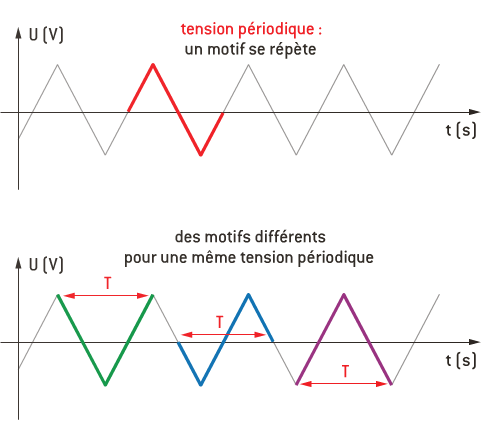
\includegraphics[scale=0.7]{bilan3}
	\end{center}

	\begin{itemize}
		\item Une tension est \kw{périodique} lorsque ses \kw{variations se répètent} identiques à elles mêmes au cours du temps. 
		\item La \kw{durée} d'un motif est la \kw{période}. On la note $T$, son unité est la seconde $s$.
	\end{itemize}
	}

\end{mybilan}

\begin{myexos}
	\begin{itemize}
		\item \exo{14}{41} : évolution de la solubilité du sel dans l'eau, en fonction de la température.
		\item \exo{15}{41} : préparation d'eau de chaux, solubilité de la chaux éteinte dans l'eau.
		\item \exo{13}{41} : QCM sur documents, sucre dans le thé : fusion vs dissolution.		
	\end{itemize}
\end{myexos}


\end{document}



%\newpage

\section{Et la température dans tout ça ?}

Le graphique ci-dessous représente la solubilité du  sel (ou chlorure de sodium) dans l'eau en fonction de la température.

\begin{questions}
	\question Complète le graphique en indiquant les grandeurs représentées en abscisse et en ordonnée.
	
	\begin{center}
		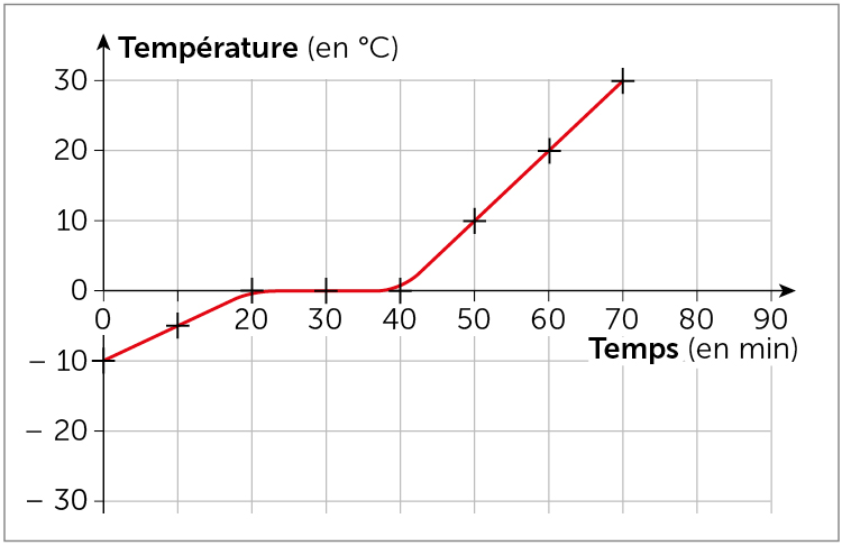
\includegraphics[scale=0.5]{img/courbe}
	\end{center}

	\question \`A $20 °C$, quelle masse de chlorure de sodium peut-on dissoudre au maximum dans 1L de solution ?
	
	\question \`A $90 °C$, quelle masse de chlorure de sodium peut-on dissoudre au maximum dans 1L de solution ?
	
	\question De quoi dépend la solubilité du sel dans l'eau ?
\end{questions}


%\newpage


\section{Quel est cet état ? (3 points)}\label{ex:etat}



\begin{questions}
	\question[3] Pour chaque phrase, indiquer quel(s) état(s) est (sont) décrit(s).
	
	
	Les molécules :\\
	\begin{parts}
		\part sont proches les unes des autres et peuvent bouger les unes par rapport aux autres.
		\begin{solution}
			L'état décrit est l'état liquide.
		\end{solution}
		
		\part sont très éloignées les unes des autres.
		\begin{solution}
			L'état décrit est l'état gazeux.
		\end{solution}
		
%		\part sont ordonnées [sont liées].
%		\begin{solution}
%			L'état décrit est l'état solide.
%		\end{solution}
%		
		\part ne peuvent pas se déplacer les unes par rapport aux autres.
		\begin{solution}
			L'état décrit est l'état solide.
		\end{solution}
		
		\part se déplacent et occupent le maximum d'espace.
		\begin{solution}
			L'état décrit est l'état gazeux.
		\end{solution}
		
		\part ont un volume propre et pas de forme propre.
		\begin{solution}
			L'état décrit est l'état solide.
		\end{solution}
		
		\part sont désordonnées [sont agitées].
		\begin{solution}
			Les états décrits sont les états liquide et gazeux.
		\end{solution}
	\end{parts}
	
\end{questions}


%\newpage 

%
\section{Monnaie en cuivre }

Au cours d'une opération de nettoyage de la plage, Romain a trouvé dix pièces de monnaie en cuivre. Il les plonge dans une éprouvette à moitié remplie d'eau. La différence de volume qu'il constate est $V = 5 cm^3$, il a trouvé sur internet que la masse volumique du cuivre est $\rho _{cuivre}$ est de $\num{8.96} g/mL$.  

\begin{questions}
	\question[] Convertir le volume $V$ des pièces de cuivre en mL.
	
	\question[] Calculer la masse $m$ de ces dix pièces de cuivre.
	
\end{questions}


%\newpage 

\section{Dans quel état est cette matière}\label{ex:etat2}

\begin{center}
	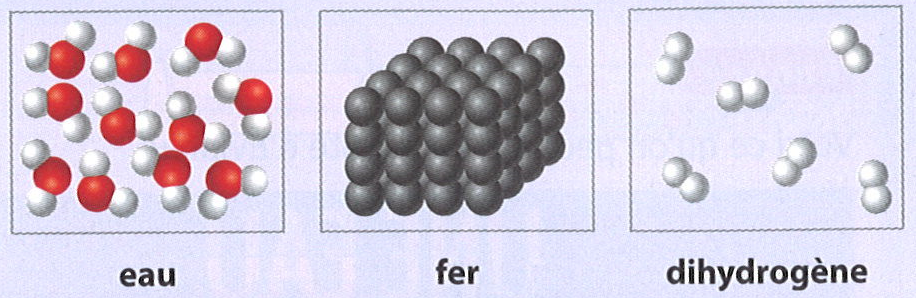
\includegraphics[scale=0.4]{img/etats}
\end{center}

\begin{questions}
\question[] Indiquer pour chacune de ces matières si elles sont dans l'état solide; liquide ou gazeux. Justifier.

\end{questions}

\section{Surface libre}\label{ex:surface}

Plusieurs récipients sont remplis à ras bord avec de l'eau liquide.


\begin{questions}
	
			
		\question[] Tracer la surface libre du liquide au repos dans chacun des récipients.
		
		\begin{center}
			
\includegraphics[scale=0.3]{img/surface}
		\end{center}	
\end{questions}


\section{Je reconnais les trois états physiques (3 poinst)}

Voici des récipients contenant des substances à l'état solide, à l'état liquide et à l'état gazeux.

\begin{questions}
	\question[3] En justifiant la réponse, indiquer l'état représenté dans chaque cas.
	%\begin{multicols}{2}
		
		\begin{center}
			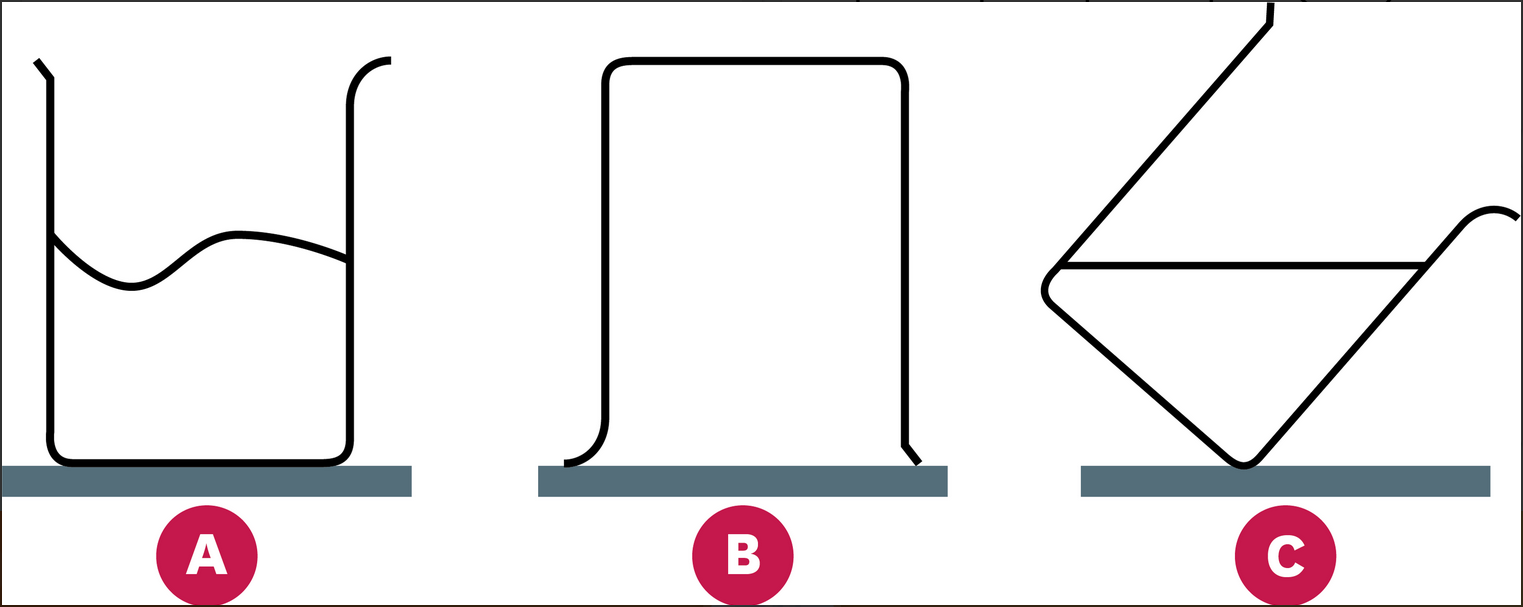
\includegraphics[scale=0.4]{img/reco1}
		\end{center}
	
	\begin{solution}
		\begin{itemize}
			\item Le contenu du bécher A n'a pas de surface libre plane donc c'est un solide.
			
			\item Le contenu du bécher B occupe tout l'espace disponible c'est un gaz.
			
			\item Le contenu du bécher C a une surface libre plane et horizontale donc c'est un liquide.
		\end{itemize}
	\end{solution}


		%\begin{center}
		%	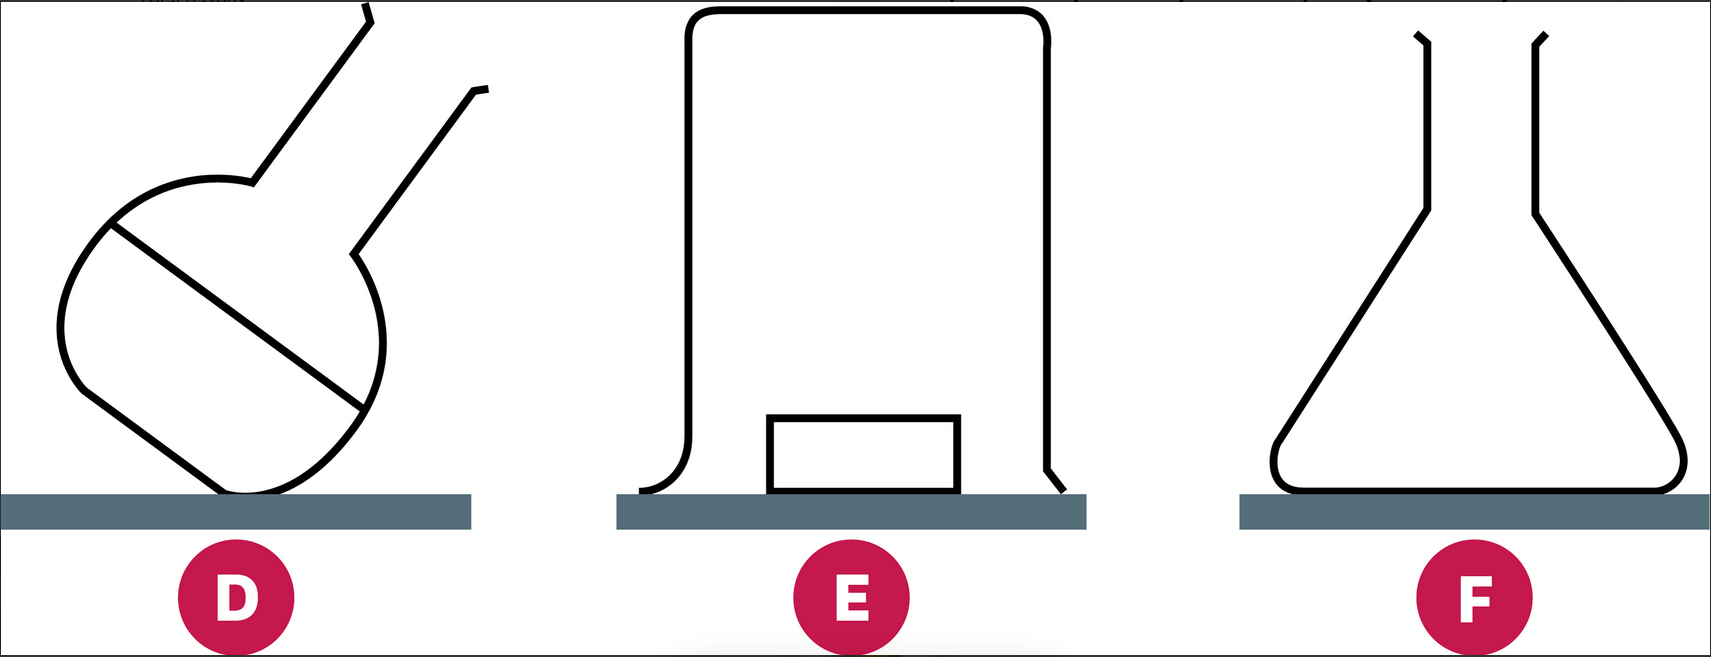
\includegraphics[scale=0.22]{img/reco2}
		%\end{center}
%		\begin{solution}
%			\begin{itemize}
%				\item Le contenu du bécher D n'a pas de surface libre horizontale donc c'est un solide.
%				
%				\item Le contenu du bécher E a une forme propre, c'est un solide.
%				
%				\item Le contenu du bécher F occupe tout l'espace disponible c'est un gaz.
%			\end{itemize}
%		\end{solution}

	%\end{multicols}
\end{questions}
 
%\newpage
%
%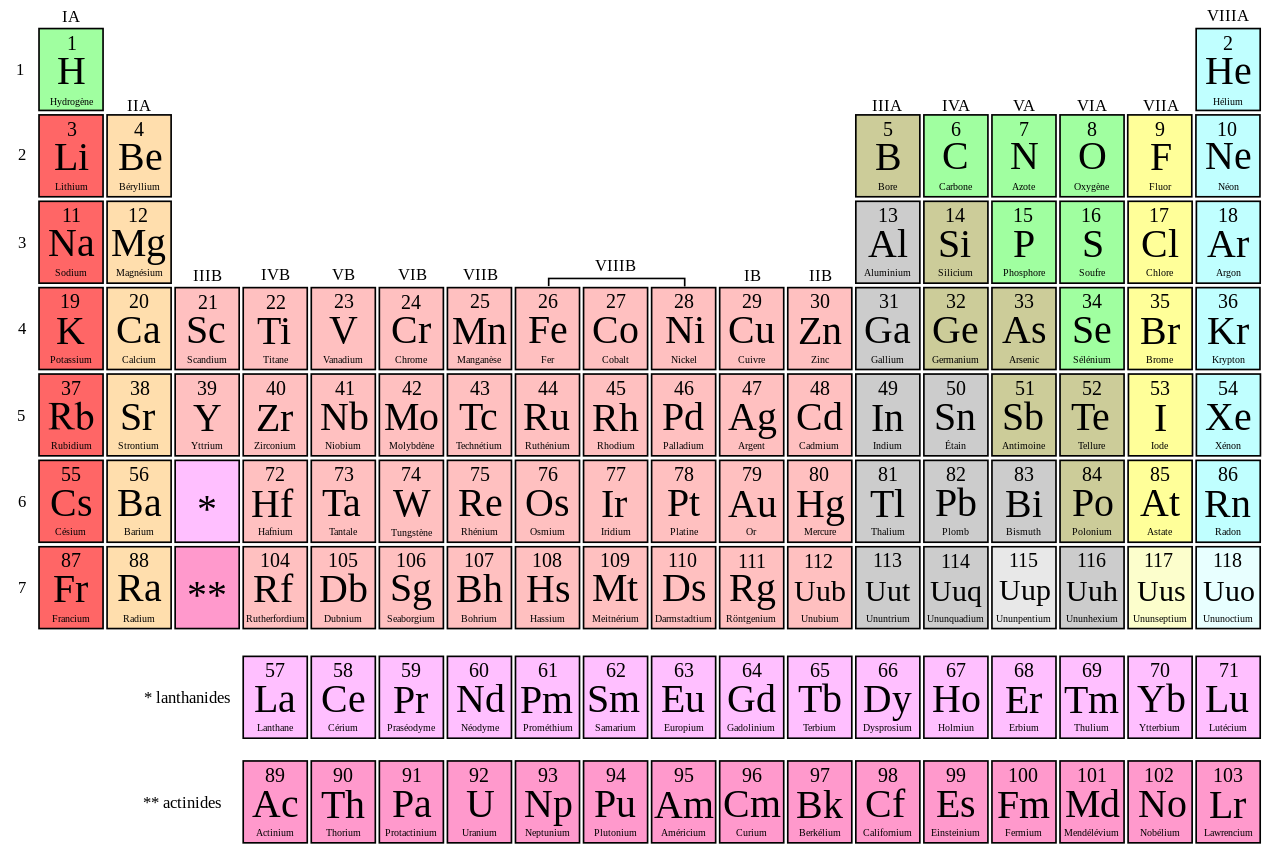
\includegraphics [scale=0.5, angle= 90 ]{img/tableau} 
\ \label{LastPage}

\end{document}